% -*- root: ../main.tex -*-
\chapter{Analisi dei Requisiti}
In questa fase sono stati individuati i \textbf{requisiti} del sistema, partendo da una descrizione di \textbf{alto livello}, ottenuta mettendosi nei panni di un committente, e procedendo con un \textbf{raffinamento} che ha portato alla definizione di requisiti più \textbf{specifici}, \textbf{chiari} e \textbf{strutturati}. 
  

	\section{Requisiti di Business}
	Si definiscono di seguito i requisiti che dovrà avere il sistema visti ad un \textbf{alto livello} di astrazione e le \textbf{aspettative} di un potenziale committente sul risultato finale.
	\begin{itemize}
	    \item Il sistema dovrà essere una replica del gioco arcade \textbf{Motos} (by Namco).
            \begin{itemize}
                \item Il gioco si svolge all'interno di un \textbf{piano} immerso nello spazio, che rappresenta il campo di gioco. All'interno del piano si muovono delle \textbf{navicelle}.
                
                \item Il giocatore ha il \textbf{comando} di una delle navicelle e ha l'obiettivo di spingere tutte le navicelle nemiche \textbf{fuori} dal campo attraverso \textbf{collisioni} che generano urti elastici.
                
                \item Sul campo sono presenti altre entità, al di fuori delle navicelle, che permettono all'utente di ottenere dei \textbf{power-up}.
                
                \item  Il giocatore ottiene una \textbf{vittoria} se non sono più presenti navicelle nemiche sull'arena e va incontro alla \textbf{sconfitta} se esce \textbf{fuori} dalla griglia per distrazione o perché spinto da un'altra navicella.
            \end{itemize}
        
        \item Il sistema dovrà mettere a disposizione un \textbf{menu} che permetta:
            \begin{itemize}
                \item La selezione della \textbf{difficoltà} di gioco
                
                \item La possibilità di modificare il \textbf{volume} e \textbf{attivare/disattivare} la musica di sottofondo
                
                \item La visualizzazione della lista dei \textbf{punteggi migliori} ottenuti nelle partite precedenti.
                
                \item La scelta della \textbf{modalità} di gioco
            \end{itemize}
            
        \item Il sistema dovrà permettere all'utente di usufruire di un \textbf{gioco piacevole}, senza interruzioni involontarie, ritardi nelle azioni e altri elementi che possano rovinare l'esperienza di gioco.
	\end{itemize}
    
    
	\section{Requisiti Utente}
	Per l'utente dovrà essere possibile svolgere le seguenti attività:
	\begin{itemize}

    	    \item Interagire con il sistema tramite un'\textbf{interfaccia grafica} intuitiva;
    	    \item \textbf{Giocare:}
    	        \begin{itemize}
            	    \item Avviare una sessione di gioco \textbf{single-player};
            	    \item Avviare una sessione di gioco \textbf{multi-player}
            	        \begin{itemize}
            	            \item selezionare un server a cui connettersi;
            	        \end{itemize}
            	   \item Scegliere ad ogni partita la \textbf{difficoltà} di gioco;
            	   \item \textbf{Giocare} attivamente inviando al sistema appositi \textbf{comandi};
    	        \end{itemize}
    	   \item Accedere alle \textbf{impostazioni} e modificarle;
    	   \item Visualizzare le \textbf{statistiche} di gioco.
	\end{itemize}
	
	\begin{figure}[H]
		\centering
		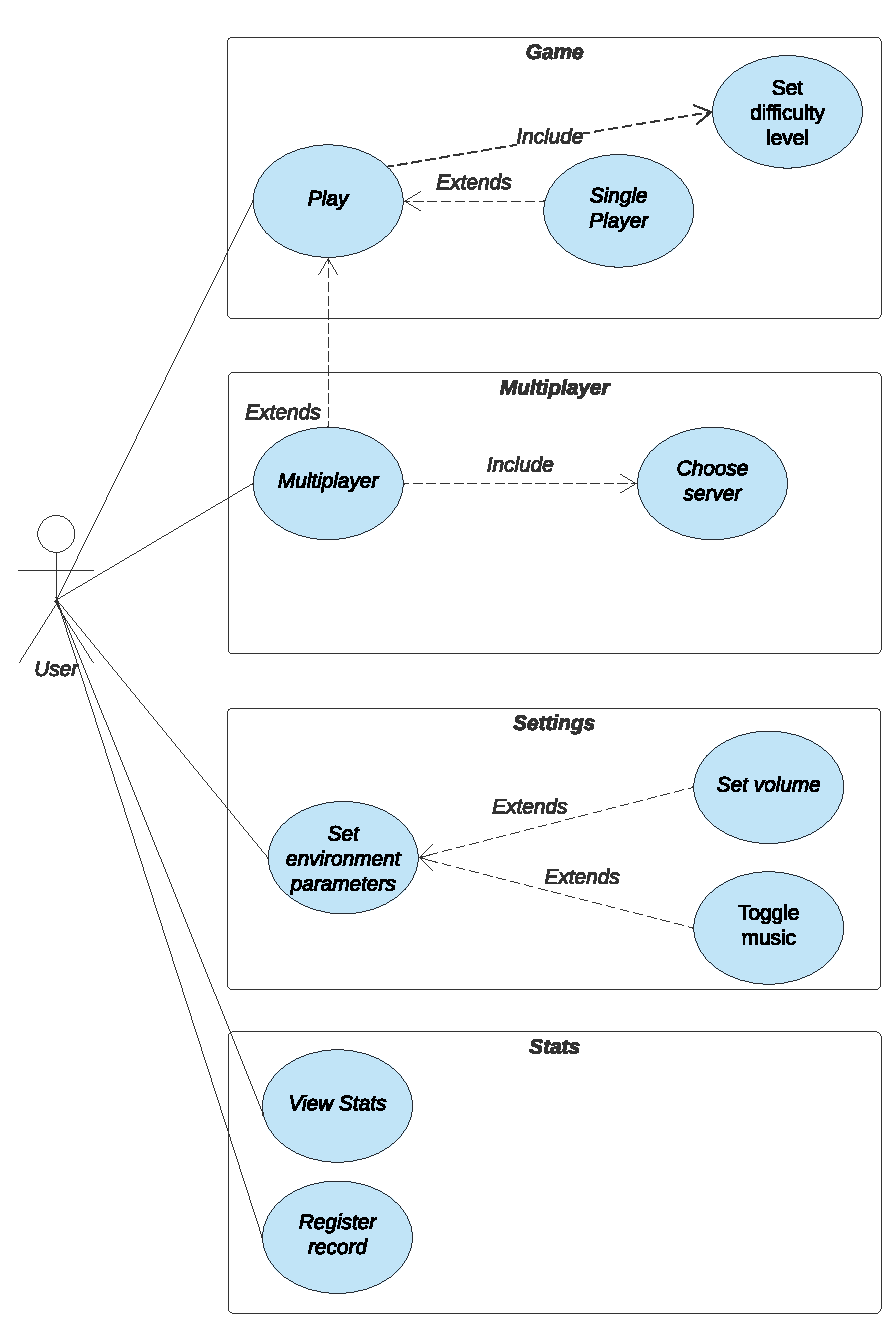
\includegraphics[width=0.80\columnwidth]{Diagrams/useCaseDiagram}
		\caption{Diagramma dei casi d'uso che evidenzia le operazioni che dovranno poter essere svolte dall'utente}
		\label{fig:figure1}
	\end{figure}

	
	\section{Requisiti Funzionali}
	Si elencano i requisiti funzionali per ognuno dei seguenti macro-componenti:
	\begin{itemize}
	    \item Gioco
	    \item Multiplayer
	    \item Impostazioni
	    \item Statistiche
	\end{itemize}

    \subsection{Gioco}
        Il gioco deve rispecchiare le meccaniche di base dell'originale. Sono presenti diverse entità, ognuna con caratteristiche specifiche:
            \begin{itemize}
                \item \textbf{Navicella}: la navicella pilotata dal giocatore dovrà:
                    \begin{itemize}
                        \item \textbf{Spostarsi} all'interno del campo di gioco 2D in base agli \textbf{input} ricevuti da tastiera
                        \item Avere una \textbf{massa} che influisce sull'\textbf{urto} con gli altri elementi in campo
                        \item Potersi \textbf{scontrare} con le altre navicelle generando un urto elastico che spinge entrambi e che \textbf{non} tiene conto della \textbf{velocità} (come nel gioco originale)
                        \item (opzionale) Avere una \textbf{durata vitale} che si decrementa ad ogni urto e il quale esaurimento comporta l'\textbf{eliminazione}.
                        
                    \end{itemize}
                \item \textbf{Navicella nemica}: le navicelle nemiche in campo, controllate dal sistema, dovranno:
                \begin{itemize}
                    \item Muoversi in base a \textbf{regole predefinite}. 
                    \item Avere l'obiettivo di \textbf{eliminare} la navicella del giocatore
                    \item (opzionale) Avere una \textbf{durata vitale} il quale esaurimento comporta l'eliminazione.
                    \item Seguire delle \textbf{strategie}. Un esempio di strategia potrebbe essere accerchiare la navicella dell'utente per spingerla fuori dal campo di gioco.
                \end{itemize}
                \item \textbf{Entità power-up}(opzionale): sul campo di gioco dovranno comparire degli elementi che tramite un'\textbf{interazione} con la navicella pilotata dal giocatore potranno fornirle dei \textbf{power-up}. 
                    \begin{itemize}
                        \item \textbf{Aumento della massa}: la massa influisce sull'urto; aumentandola il giocatore ottiene il vantaggio di prevalere in caso di collisione, spingendo l'oggetto più lontano.
                        \item \textbf{Aumento della velocità}: la velocità viene ignorata nel calcolo della spinta generata da una collisione, tuttavia il suo incremento può essere utile per sfuggire ai nemici più lenti.
                        \item \textbf{Vita aggiuntiva}: permette alla navicella dell'utente di guadagnare un tentativo in più in caso di sconfitta.
                        \item \textbf{Rimozione dei power-up}: reimposta la massa e la velocità a quelle di default.
                        \item \textbf{Incremento del punteggio}: è contenuto in degli elementi che possono essere spinti fuori dal campo come le navicelle e assegnano un punteggio se eliminati dal campo di gioco.
                    \end{itemize}
                \item \textbf{Giocatore}: il giocatore è l'entità principale, intorno alla quale ruotano le dinamiche di gioco. 
                    \begin{itemize}
                        \item Il giocatore può \textbf{controllare} una navicella
                        \item Accumula \textbf{punti} eliminando le altre navicelle e, opzionalmente, interagendo con le entità power-up
                        \item Ha un determinato numero di \textbf{vite}, che rappresentano il numero di volte in cui si può riprendere il gioco dopo essere stati eliminati, senza che venga fatto un \textbf{reset} dello stato
                        \item Ha l'obiettivo di \textbf{eliminare} le navicelle nemiche 
                    \end{itemize}
                \item \textbf{Arena di gioco}: è lo \textbf{spazio} su cui si muovono gli elementi del gioco.
                \begin{itemize}
                    \item Si compone di un piano \textbf{bidimensionale} suddiviso da una \textbf{griglia} che rappresenta le \textit{piastrelle} dell'arena.
                    \item (opzionale) L'arena può presentare al suo interno delle \textit{piastrelle} \textbf{mancanti} che non fanno parte del campo di gioco e che comportano quindi l'eliminazione delle navicelle che le attraversano.    
                    \item Ha dei \textbf{bordi} ben definiti che la delimitano dall'area circostante e che se attraversati da una navicella ne comportano l'eliminazione.
                \end{itemize}
            \end{itemize}
        \subsection{Multiplayer}
            Opzionalmente il gioco sarà fruibile anche in modalità \textbf{Multiplayer}. 
            La modalità Multiplayer dovrà permettere a \textbf{più giocatori} di interagire all'interno della \textbf{stessa arena}.\\
            Il multiplayer potrà essere di \textbf{due tipi}:
            \begin{itemize}
                \item \textbf{Cooperativo}: i giocatori sono \textbf{alleati} e hanno l'obiettivo di eliminare le navicelle pilotate dal sistema. 
                \begin{itemize}
                    \item  Le condizioni di \textbf{vittoria} saranno:
                        \begin{itemize}
                            \item \textbf{Eliminazione} delle navicelle \textbf{nemiche}
                            \item \textbf{Sopravvivenza} di almeno una delle navicelle \textbf{alleate}.
                        \end{itemize}
                    
                     \item  I giocatori andranno incontro alla \textbf{sconfitta} se:
                        \begin{itemize}
                            \item Sul campo rimangono \textbf{solo} le navicelle nemiche
                        \end{itemize}
                \end{itemize}
                
                \item \textbf{Competitivo}: i giocatori sono \textbf{avversari} e ognuno di loro ha l'obiettivo di rimanere l'\textbf{unica} navicella sul campo. 
                \begin{itemize}
                    \item  Le condizioni di \textbf{vittoria} saranno:
                        \begin{itemize}
                            \item \textbf{Eliminazione} delle navicelle pilotate dal \textbf{sistema}.
                            \item \textbf{Eliminazione} delle navicelle pilotate da altri \textbf{giocatori}.
                        \end{itemize}
                    
                     \item  I giocatori andranno incontro alla \textbf{sconfitta} se:
                        \begin{itemize}
                            \item La navicella da loro pilotata \textbf{esce} dal campo di gioco
                            \item (opzionale) I \textbf{punti vita} della loro navicella arrivano a \textbf{
    zero} per aver subito danni
                        \end{itemize}
                \end{itemize}
            \end{itemize}
        
        \subsection{Impostazioni}
            Deve essere prevista la possibilità di gestire le impostazioni che riguardano l'ambiente dentro il quale si trova il gioco.\\
            Le \textbf{impostazioni} disponibili saranno le seguenti:
            \begin{itemize}
                \item \textbf{Musica}: deve essere possibile \textbf{attivare} o \textbf{disattivare} la musica di sottofondo.
                \item \textbf{Volume}: l'utente deve poter \textbf{regolare} il volume della musica di sottofondo.
            \end{itemize}
            
        \subsection{Statistiche}    
            Dovranno essere disponibili delle statistiche, basate sulle \textbf{partite precedenti} in modalità single player.
            Le statistiche dovranno mostrare i \textbf{record} raggiunti dai giocatori; in particolare verranno visualizzate le seguenti informazioni: 
            \begin{itemize}
                \item \textbf{Posizione} in classifica.
                \item \textbf{Username} dell'utente che detiene quel record.
                \item \textbf{Punteggio} totalizzato in quella circostanza.
            \end{itemize}
            Alla vittoria da parte di un giocatore, nel caso in cui il suo punteggio gli consentisse il piazzamento in classifica, avrà l'opzione di inserire il suo nome utente, al fine di registrare il punteggio in classifica.

            
	\section{Requisiti non Funzionali}
        Il sistema dovrà rispettare alcuni requisiti non funzionali che ne determineranno la \textbf{qualità}:
        \begin{itemize}
            \item \textbf{Reattività}: l'utente non deve percepire \textbf{ritardi} tra l'invio di un comando e l'esecuzione dello stesso da parte del gioco, il feedback grafico deve essere immediato.
            
            \item \textbf{Prestazioni}: devono essere tenute particolarmente in considerazione le \textbf{performance} affinché il gioco risulti fluido.
            
            \item \textbf{Scalabilità}: in caso venga gestita la modalità multiplayer, il gioco deve essere \textbf{scalabile} per poter supportare la gestione più client.
            
            \item \textbf{Fault tollerance}: la \textbf{gestione degli errori} deve essere adeguatamente implementata affinché le interruzioni involontarie del gioco avvengano solo in casi particolari.
            

        \end{itemize}
	\section{Requisiti Implementativi}
    \subsection{Client}
    \subsection{Server}